\documentclass[catalan, a4paper, nobib]{tufte-handout}

% encoding
\usepackage[utf8]{inputenc}
\usepackage[T1]{fontenc}
\usepackage{lmodern}
\usepackage{babel}

\frenchspacing
\usepackage[style=spanish]{csquotes}
\MakeAutoQuote{«}{»}

\usepackage{booktabs}
\usepackage{circuitikz}
\usepackage{siunitx}
\usepackage{amsmath}

\graphicspath{
    {fotos/}
}

% hyperlink setup / metadata
\usepackage{hyperref}
\AfterPreamble{\hypersetup{
  %%pdfauthor={},
  %%pdftitle={},
  %%pdfsubject={},
}}

% document metadata
\author{Sofija Starcevic i Víctor Méndez}
\title{FISE: Pràctica 1}
\date{19-2-2024}

\begin{document}

\maketitle

\newthought{Qüestió 1.1:} El GF mostra \qty{5}{\volt} de pic a pic. L'osci\l.loscopi mostra \qty{10}{\volt}. No coincideixen.

\newthought{Qüestió 1.2:} Els dos aparells mostren \qty{10}{\volt}.

\newthought{Qüestió 1.3:} Entre \qty{1}{\ohm} i \qty{10}{\kilo\ohm}. Per defecte \qty{50}{\ohm}. El circuit equivalent es veu a la figura \ref{fig:circ_equiv}.

\begin{marginfigure}
  \begin{center}
    \begin{circuitikz}[american voltages]
      \draw (0,0) to[short, o-] ++(-1,0) to[R=$R_G$] ++(-2,0) to[short] ++(-1,0) to[V=$V_G$] ++(0,-2) to[short, -o] ++(4,0);
      \draw (0,0) to[open, v^>=$V_o$] ++(0,-2);
    \end{circuitikz}
  \end{center}
  \caption{Circuit equivalent del generador}
  \label{fig:circ_equiv}
\end{marginfigure}

\newthought{Questió 1.4:} El circuit equivalent amb càrrega es veu a la figura \ref{fig:circ_equiv_load}. L'expressió és $V_G = V_o(1+\frac{R_G}{R_L})$.

\begin{marginfigure}
  \begin{center}
    \begin{circuitikz}[american voltages]
      \draw (0,0) to[short, o-] ++(-1.5,0) to[R=$R_G$] ++(-1.5,0) to[short] ++(-0.5,0) to[V=$V_G$] ++(0,-2) to[short, -o] ++(3.5,0);
      \draw (0,0) to[open, v^>=$V_o$] ++(0,-2);
      \draw (-1,0) to[R=$R_L$] ++(0,-2);
    \end{circuitikz}
  \end{center}
  \caption{Circuit equivalent del generador amb càrrega}
  \label{fig:circ_equiv_load}
\end{marginfigure}

\newthought{Qüestió 1.5:} La resistència d'entrada és \qty{10}{\mega\ohm}. Aquesta és molt més gran que els \qty{50}{\ohm} del generador i, per tant, tota la tensió $V_G$ cau al osci\l.loscopi. Això explica la disparitat de mesures.

\newthought{Qüestió 1.6:} El voltatge que caurà a la carrega no serà el desitjat i la potència a la carrega no serà màxima.

\newthought{Qüestió 1.7:} Veure figura \ref{fig:circ_equiv_load2}. El GF s'hauria de configurar a \qty{100}{\ohm}.

\begin{marginfigure}
  \begin{center}
    \begin{circuitikz}[american voltages]
      \draw (0,0) to[short] ++(-1.5,0) to[R=\qty{50}{\ohm}] ++(-1.25,0) to[short] ++(-0.5,0) to[V=$V_G$] ++(0,-2) to[short] ++(3.25,0);
      \draw (0,0) to[R=\qty{10}{\mega\ohm}] ++(0,-2);
      \draw (-1.25,0) to[R=\qty{100}{\ohm}] ++(0,-2);
    \end{circuitikz}
  \end{center}
  \caption{Circuit equivalent del generador amb una càrrega de \qty{100}{\ohm}}
  \label{fig:circ_equiv_load2}
\end{marginfigure}

\newthought{Qüestió 1.8:} Veure figura \ref{fig:foto1}. Es correspon tot.

\newthought{Qüestió 1.9:} Primer es selecciona el tipus d'ona, amplitud i freqüència com sempre. Després es prem el botò burst i es selecciona els cicles i el periode de burst.

\newthought{Qüestió 1.10:} El senyal desapareix. Si posem el trigger massa alt l'osci\l.loscopi no dispara.

\newthought{Qüestió 1.11:} El trigger li fa saber al osci\l.loscopi quan disparar. Si no es configura no es veu be el senyal o es pot veure desfasat.

\newthought{Qüestió 1.12:} L'osci\l.loscopi emmagatzema dades fins que el senyal supera el llindar del trigger amb la pendent que toca. En aquest moment continua prenent dades fins emplenar el buffer i finalment mostra el senyal.

\newthought{Qüestió 1.13:} Si només s'indica el llindar de voltatge hi ha dues maneres diferents d'adquirir el mateix senyal. Un cop determinat el pendent fixem la manera de disparar el senyal.

\newthought{Qüestió 1.14:} Veure la figura \ref{fig:foto2}.

\newthought{Qüestió 1.15:} Veure la figura \ref{fig:foto3}. Es correspon.

\newthought{Qüestió 1.16:} Segons la formula $TOF = \frac{2d}{v} = \frac{2(0.25)}{343} \simeq \qty{1.5}{\milli\second}$.

\newthought{Qüestió 1.17:} Veure la figura \ref{fig:foto4}.

\newthought{Qüestió 1.18:} El temps mesurat és $\simeq \qty{1.6}{\milli\second}$ que correspon a una distància $d\simeq\qty{27}{\centi\meter}$.

\newthought{Qüestió 1.19:} La amplitud màxima és \qty{175}{\milli\volt}.

\newthought{Qüestió 1.20:} L'amplitud de l'eco es màxima per $f_{op}=\qty{40}{\kilo\hertz}$.

\begin{figure}
  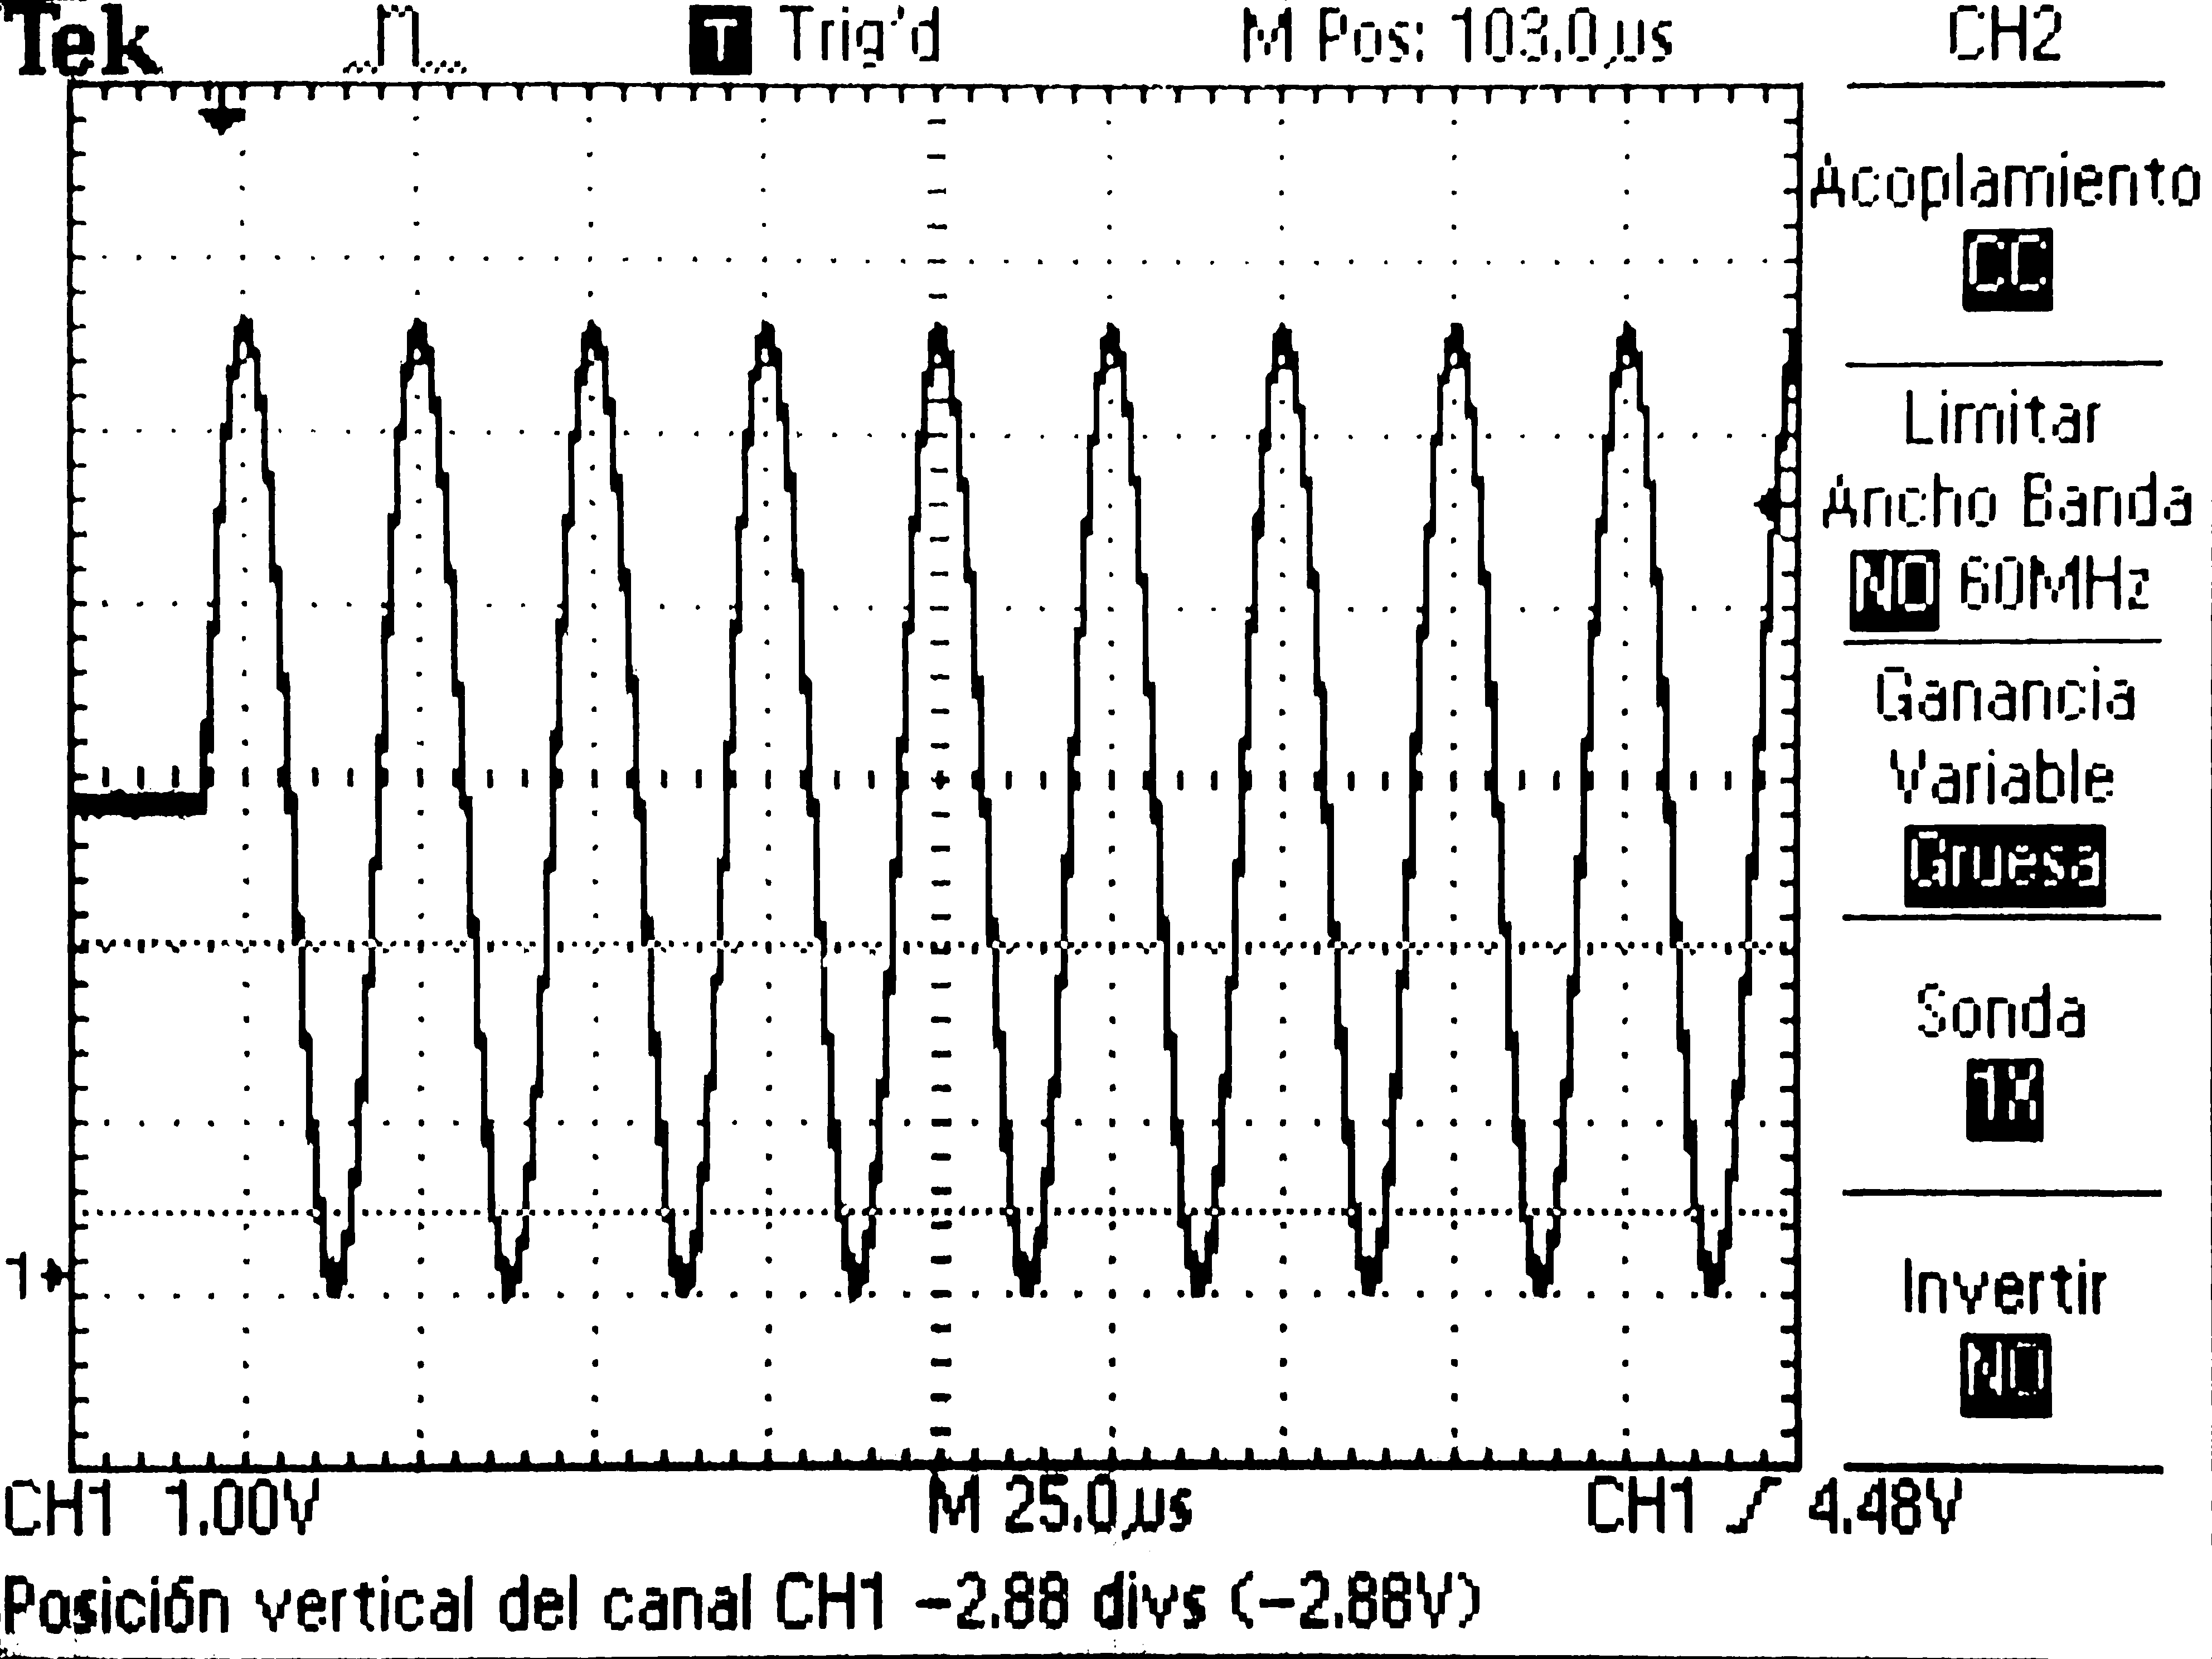
\includegraphics[width=\linewidth]{foto1.png}
  \caption{Sinusoide generada pel GF}
  \label{fig:foto1}
\end{figure}

\begin{figure}
  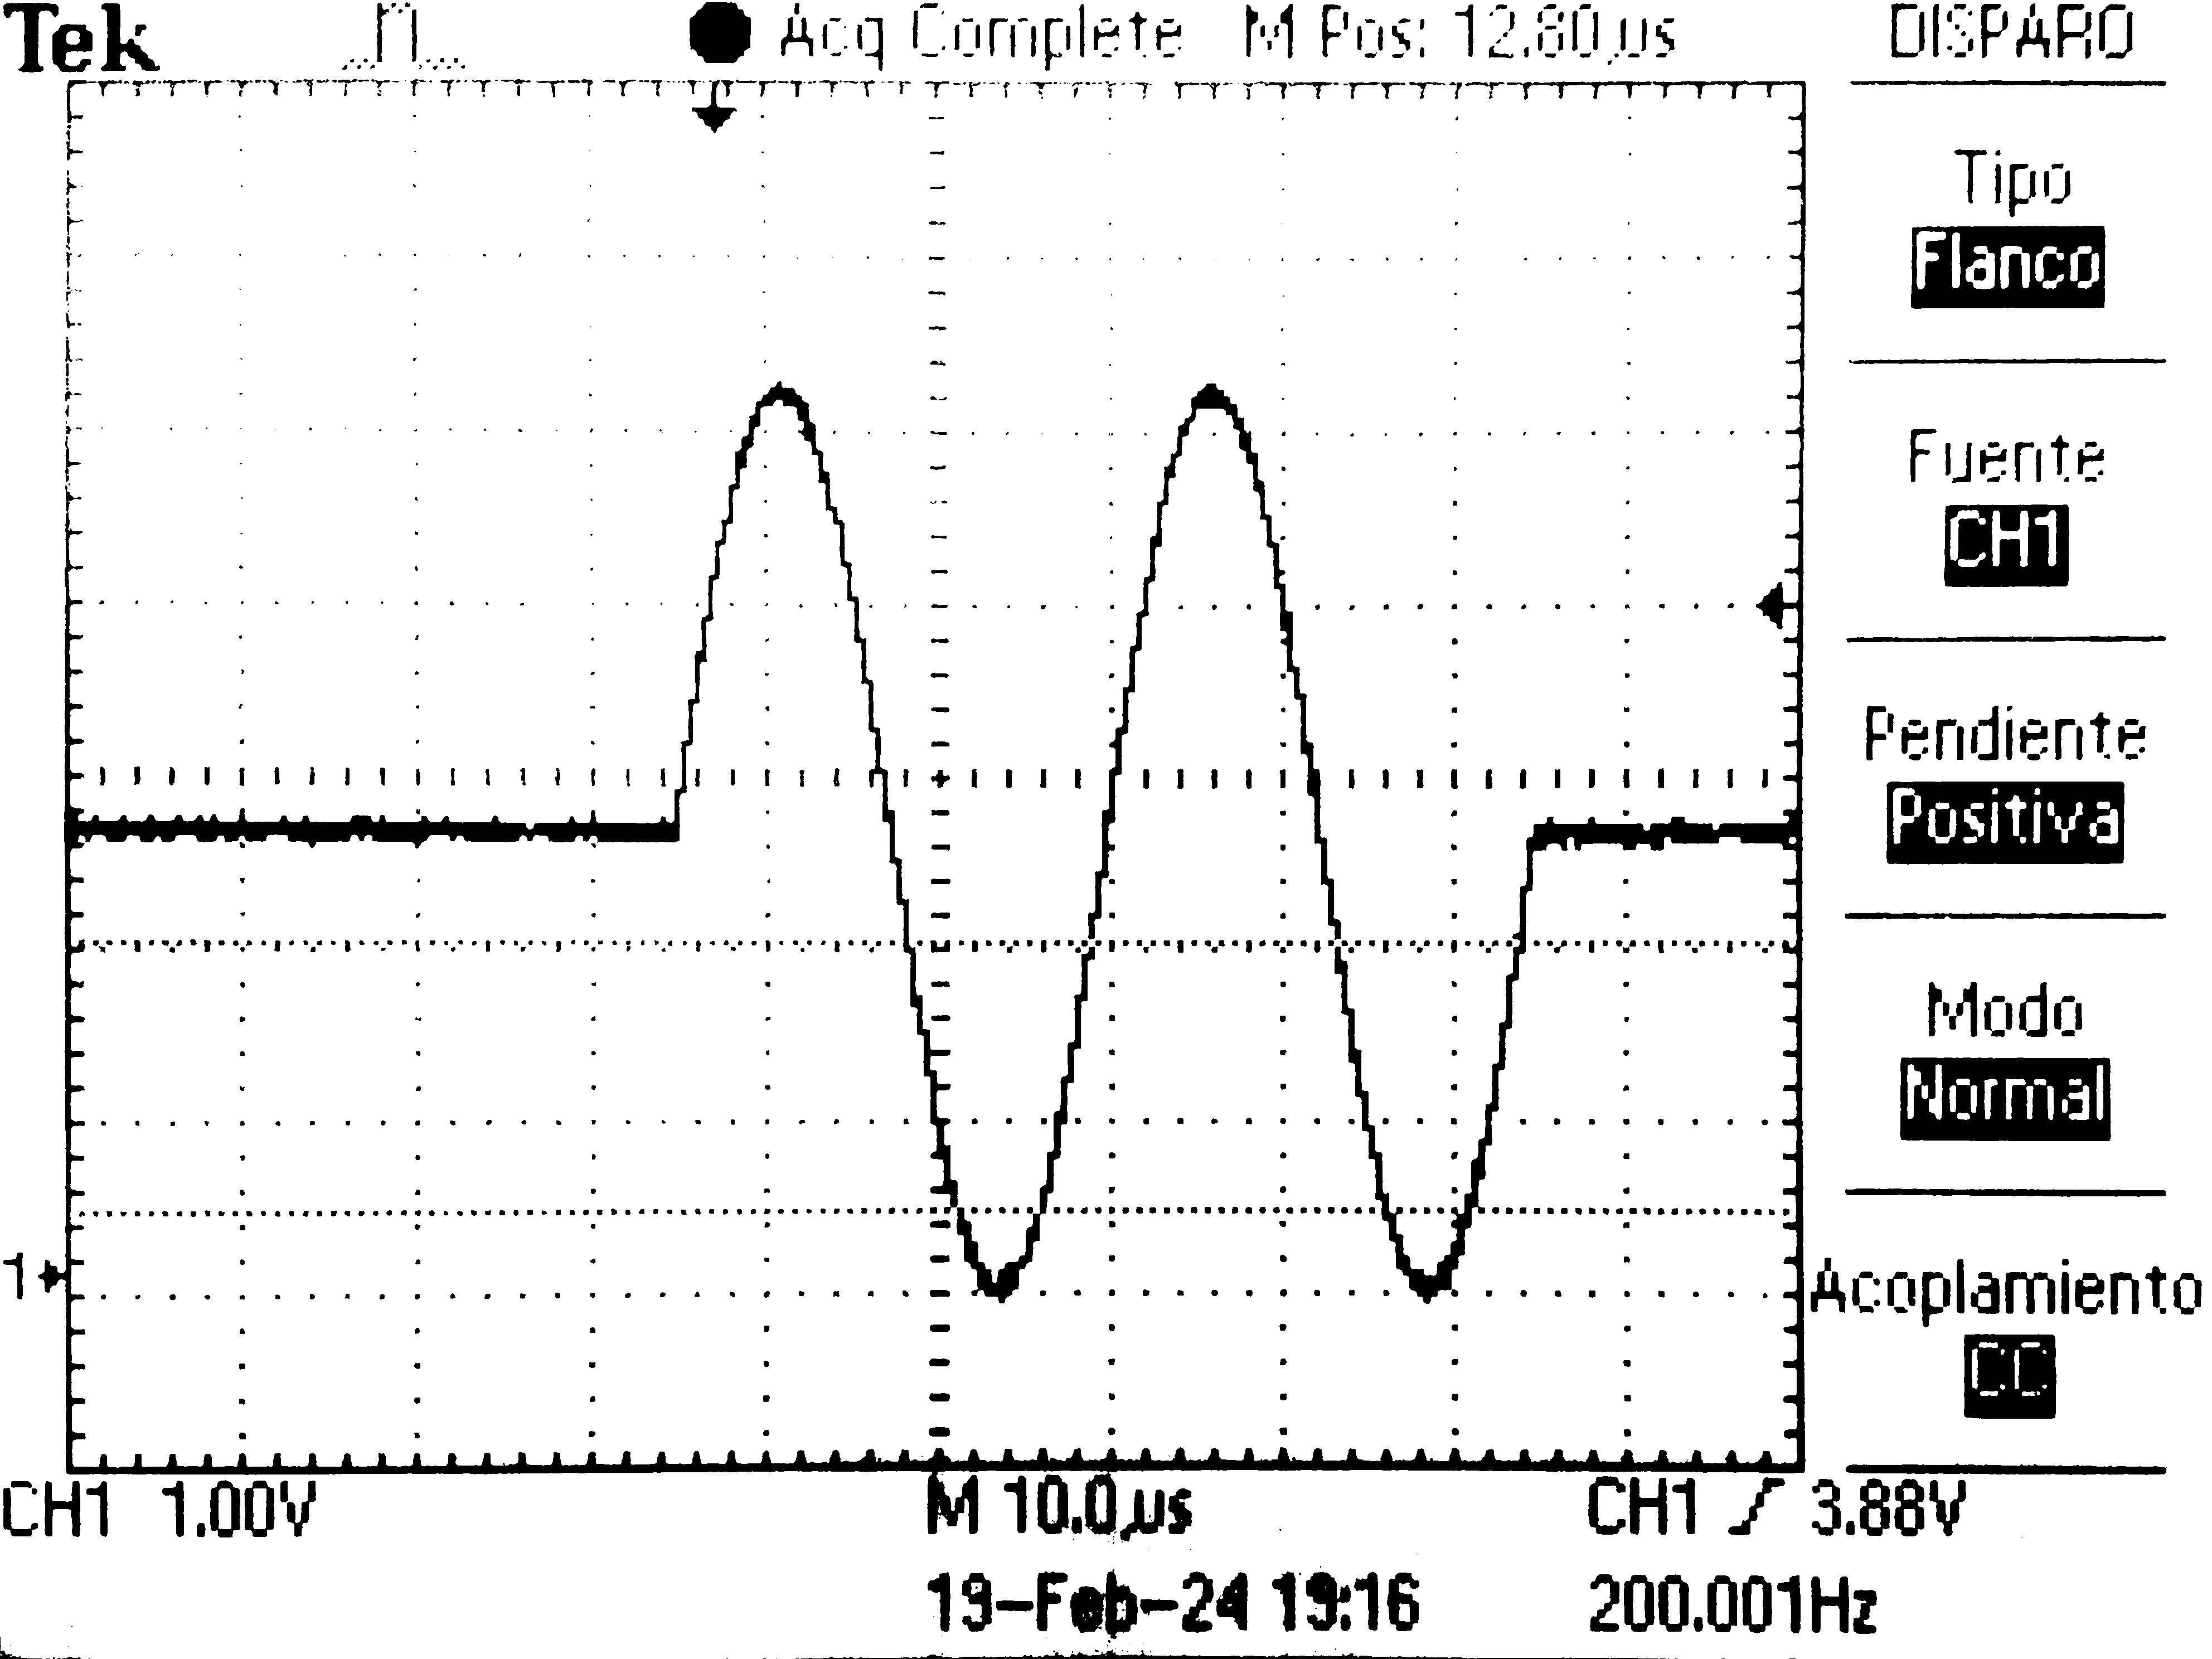
\includegraphics[width=\linewidth]{foto2.png}
  \caption{Ràfaga del GF}
  \label{fig:foto2}
\end{figure}

\begin{figure}
  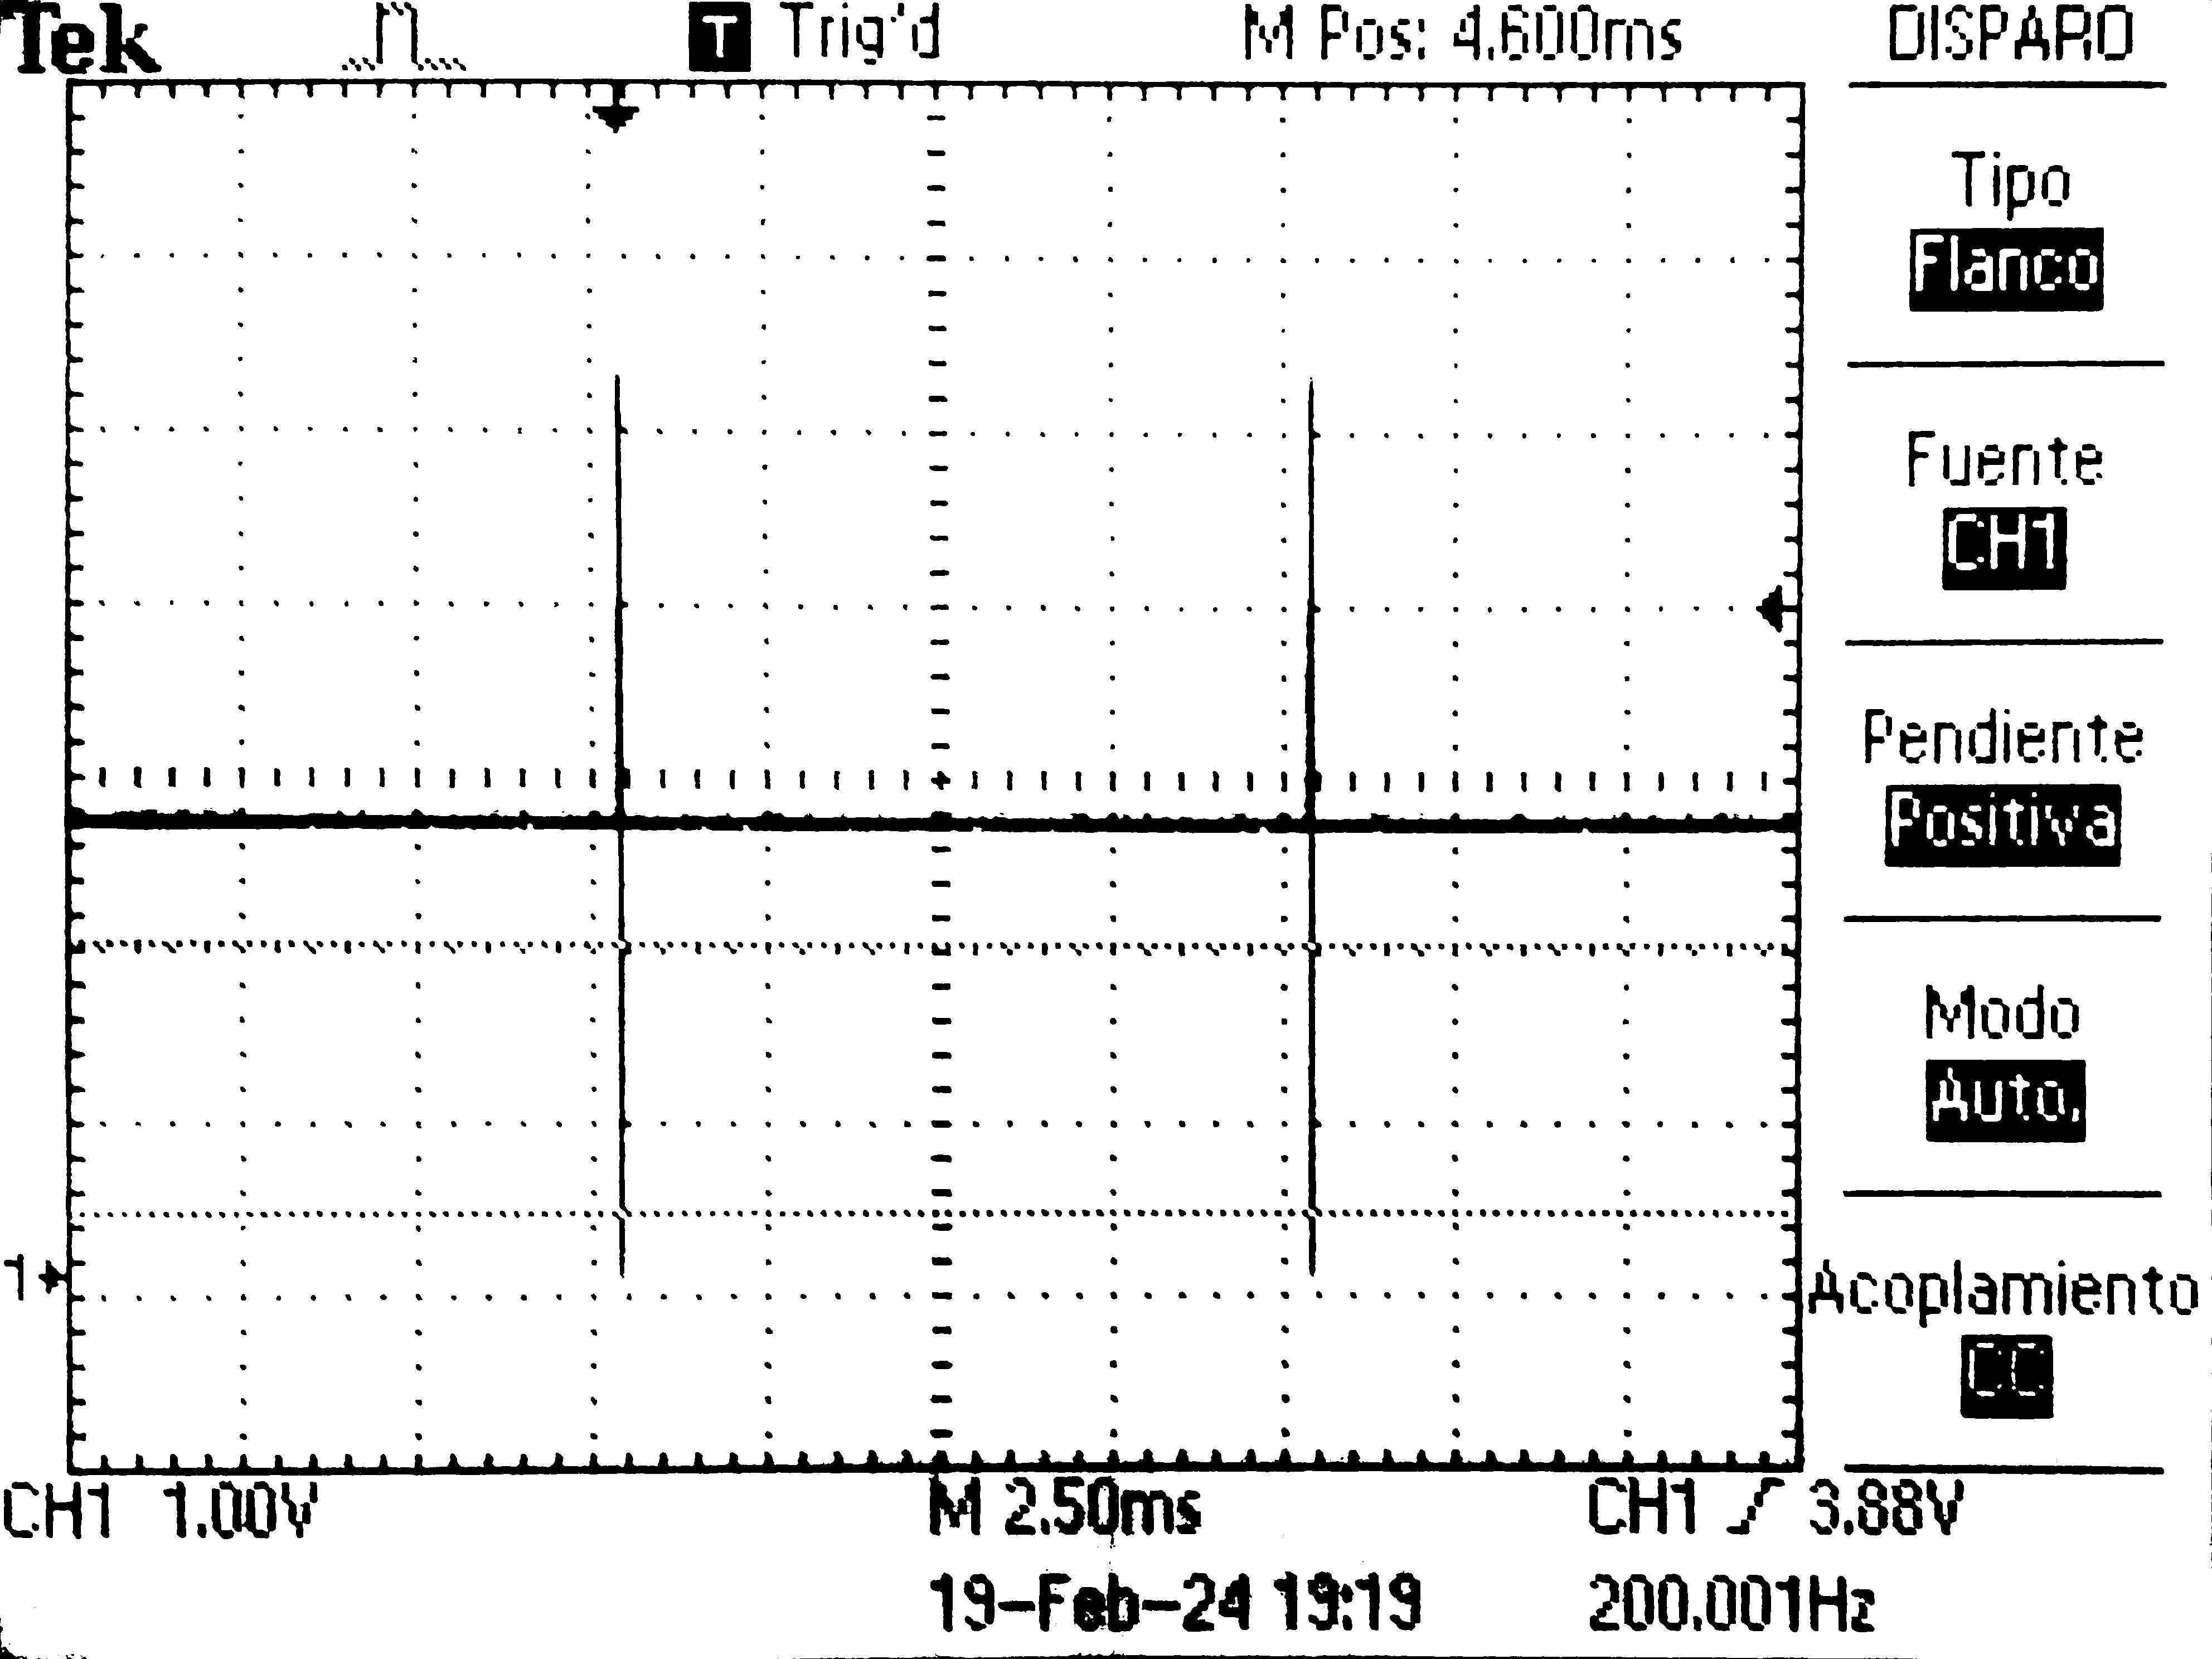
\includegraphics[width=\linewidth]{foto3.png}
  \caption{Dues ràfagues separades per \qty{10}{\milli\second}}
  \label{fig:foto3}
\end{figure}

\begin{figure}
  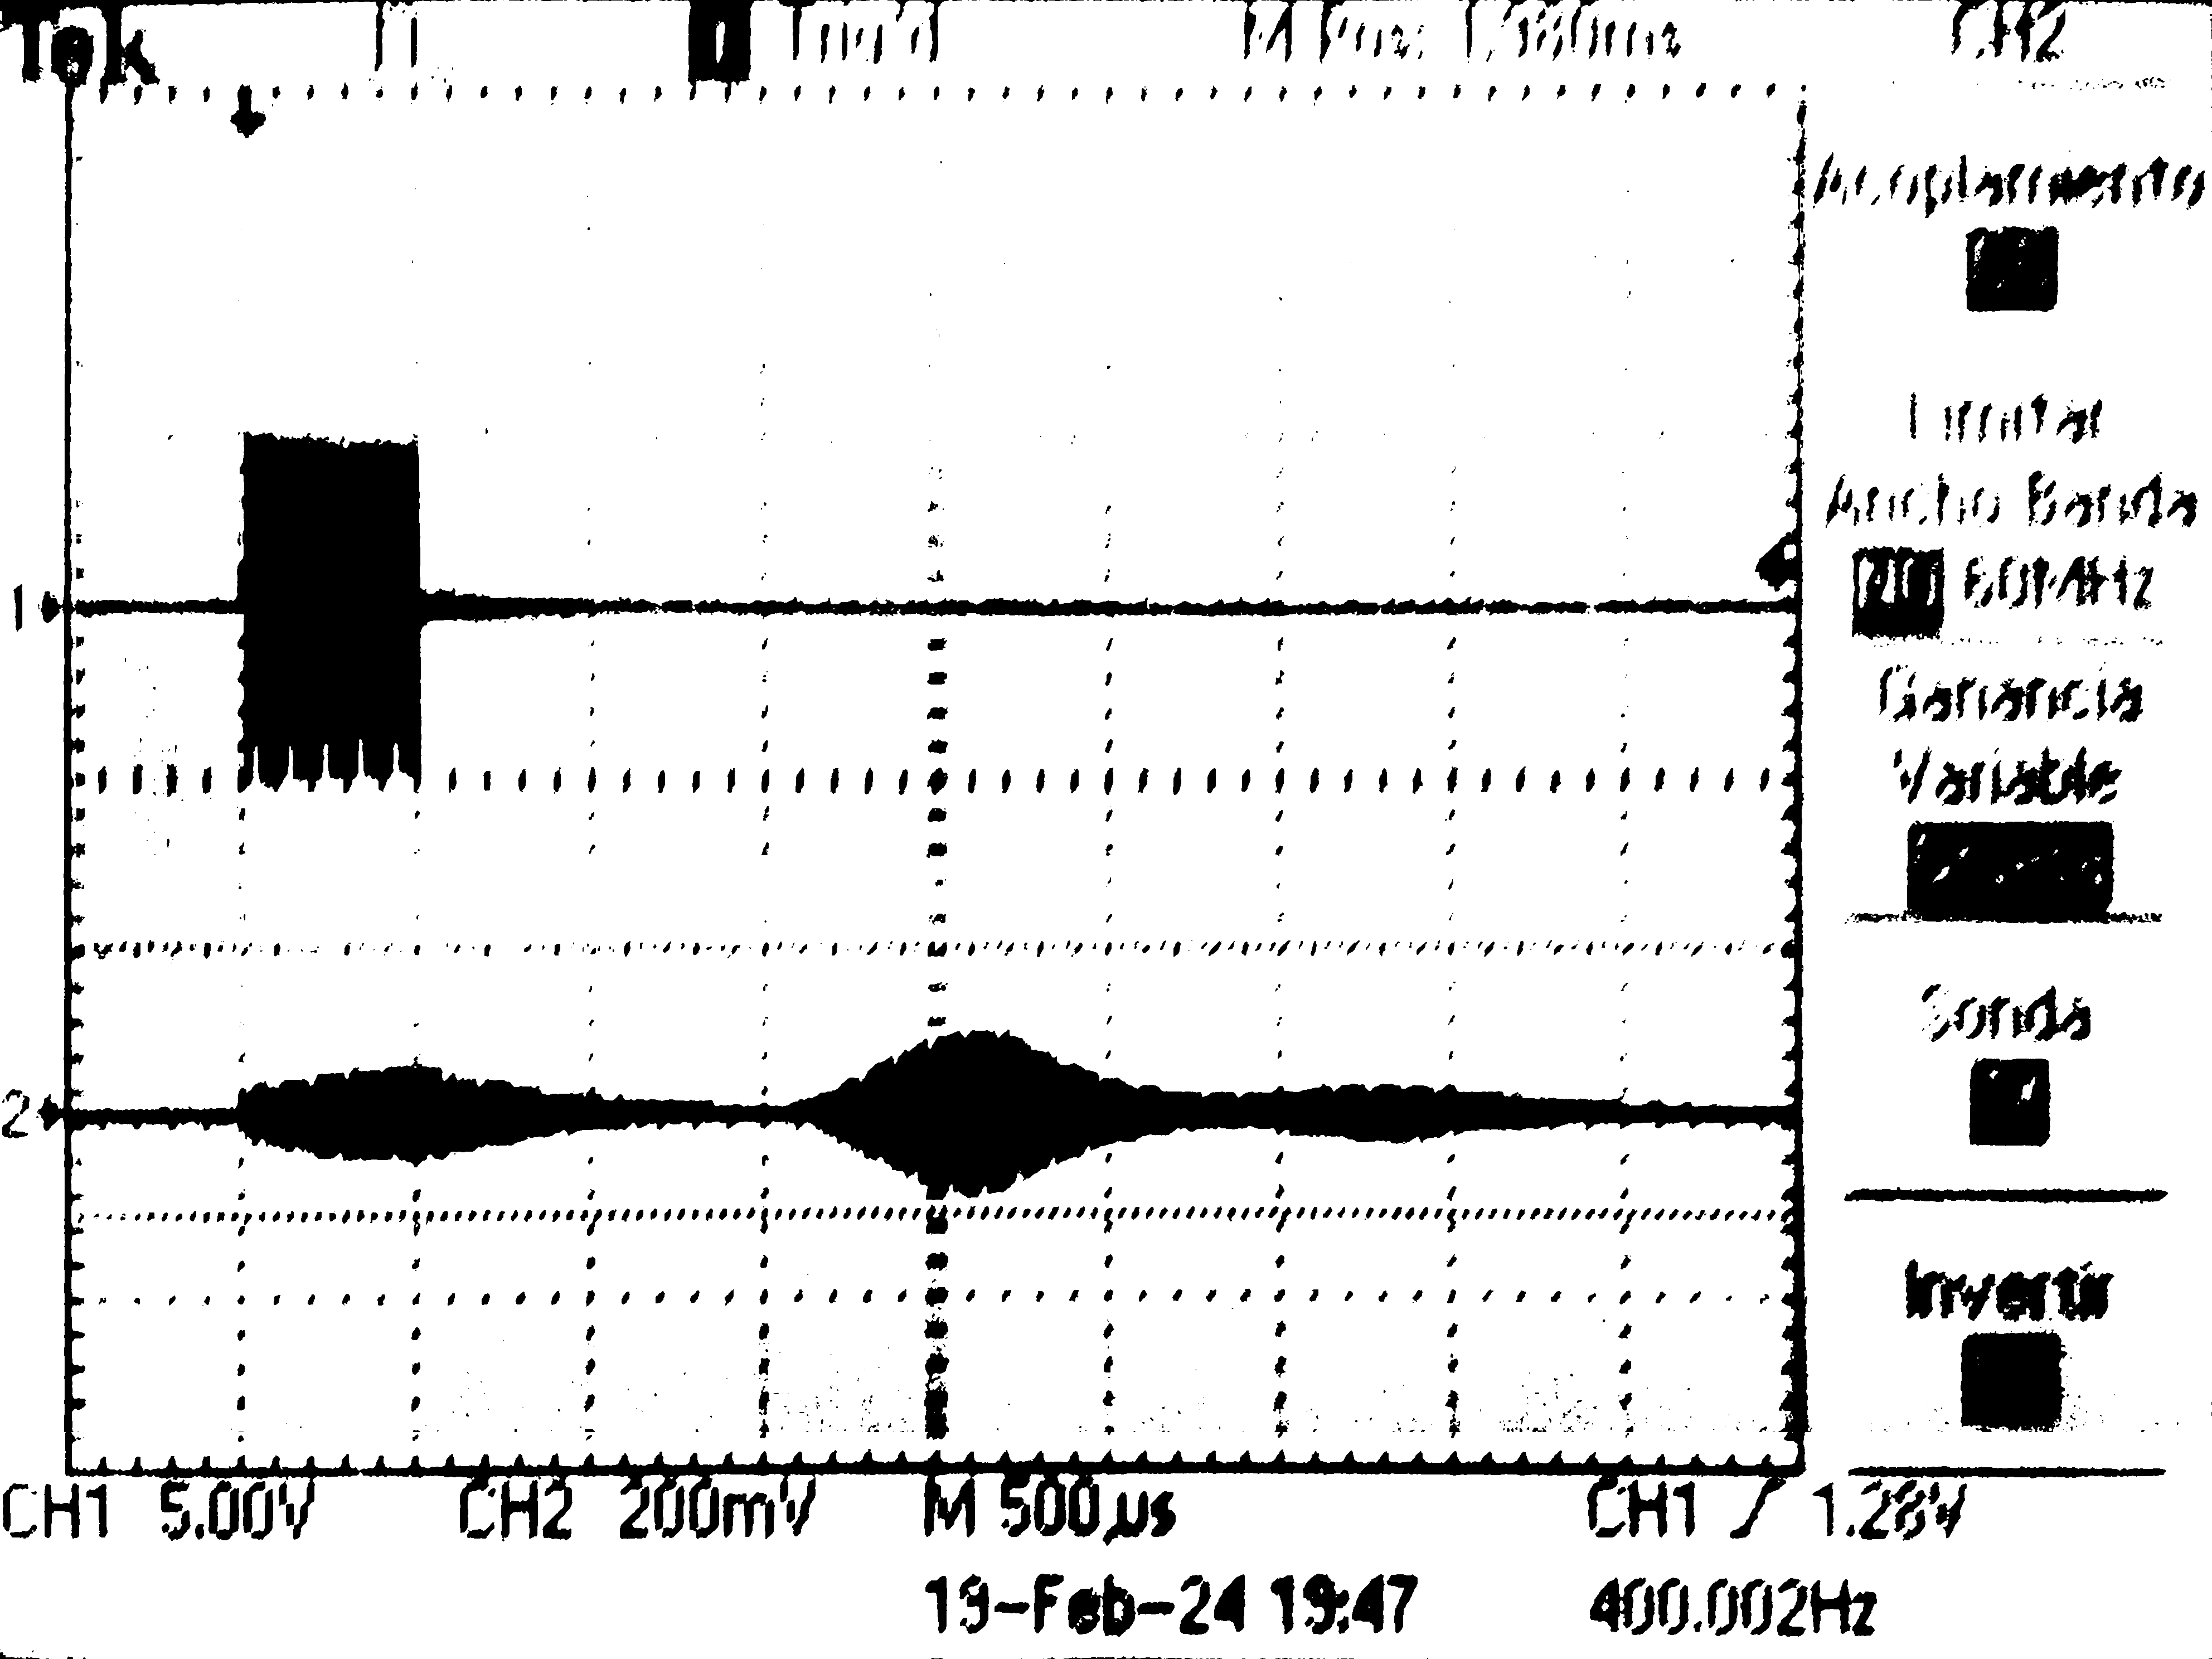
\includegraphics[width=\linewidth]{foto4.png}
  \caption{Captura de l'eco rebut}
  \label{fig:foto4}
\end{figure}

\end{document}
